On considère le cube $ABCDEFGH$ ci-dessous tel que $AB = 1$.

On note $M$ le centre de la face $BCGF$ et $N$ le centre de la face $EFGH$.

\begin{center}
	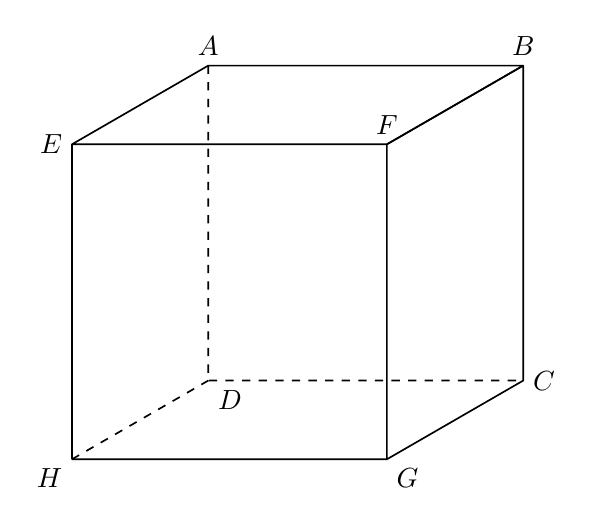
\begin{tikzpicture}[x={(0:1cm)},y={(30:0.5cm)},z={(90:1cm)},line join=bevel]
		\coordinate (H) at (0,0,0) ; \draw (H) node[below left] {$H$} ;
		\coordinate (G) at (4,0,0) ; \draw (G) node[below right] {$G$} ;
		\coordinate (C) at (4,4,0) ; \draw (C) node[right] {$C$} ;
		\coordinate (D) at (0,4,0) ; \draw (D) node[below right] {$D$} ;
		\coordinate (E) at (0,0,4) ; \draw (E) node[left] {$E$} ;
		\coordinate (F) at (4,0,4) ; \draw (F) node[above] {$F$} ;
		\coordinate (B) at (4,4,4) ; \draw (B) node[above] {$B$} ;
		\coordinate (A) at (0,4,4) ; \draw (A) node[above] {$A$} ;
		\draw[semithick,dashed] (H)--(D) (A)--(D)--(C) ;
		\draw[semithick] (H)--(G)--(C)--(B)--(F)--(G) ;
		\draw[semithick] (H)--(E)--(A)--(B)--(F)--(E) ;
	\end{tikzpicture}
\end{center}

\medskip

On se place dans le repère orthonormé $\left(D; \vect{DH},\,\vect{DC},\,\vect{DA}\right)$.

\medskip

\begin{enumerate}
	\item Donner sans justifier les coordonnées des points $F$ et $C$.
	\item Calculer les coordonnées des points $M$ et $N$.
	\item 
	\begin{enumerate}
		\item Démontrer que le vecteur $\vect{AG}$ est normal au plan $(HFC)$.
		\item En déduire une équation cartésienne du plan $(HFC)$.
	\end{enumerate}
	\item Déterminer une représentation paramétrique de la droite $(AG)$.
	\item Démontrer que le point R de coordonnées $\left(\dfrac23;\dfrac23;~\dfrac13\right)$ est le projeté orthogonal du point $G$ sur le plan $(HFC)$.
	\item On admet qu'une représentation paramétrique de la droite $(FG)$ est : \[ \begin{dcases} x=1 \\ y=1 \\ z=t \end{dcases} \: (t \in \R). \]
	%
	Démontrer qu'il existe un unique point $K$ sur la droite $(FG)$ tel que le triangle $KMN$ soit rectangle en $K$.
	\item Quelle fraction du volume du cube $ABCDEFGH$ le volume du tétraèdre $FNKM$ représente-t-il ?
\end{enumerate}